\chapter{Results}
\label{sec:results}

This chapter will present the results to the reader.


\section{Evaluation of algorithm speed}
Table 4.1 shows the end-to-end time for the lane detection system currently implemented on the Raspberry Pi. Since the lane detection system need to be run in real time the speed of the algorithm is of great importance. This measurement includes the time for the image processing steps as well as the control structure and steering signal that goes to the servo motor that controls the steering. The mean fps is calculated as 1/mean time.


\begin{table}[H]
\centering
\caption{System End-to-end time}
\label{End-to-end time}
\begin{tabular}{@{} l *4c @{}}
\toprule
Image Resolution   & & & 384x288 & 640x480  \\ 
\midrule
 Mean time & & & 0.057 & 0.0786 \\ 
 Mean fps & & & 17.54 & 12.724 \\
\bottomrule
 \end{tabular}
\end{table}



\begin{figure}[H]
  \begin{subfigure}[b]{\textwidth}
    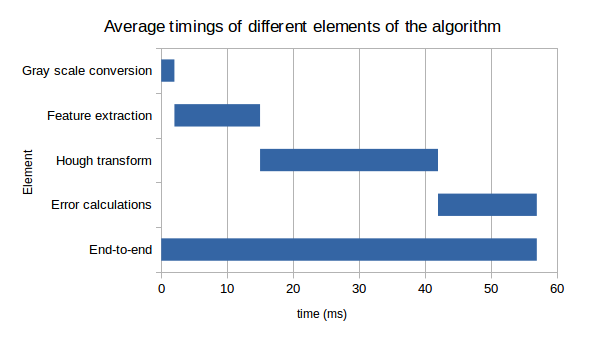
\includegraphics[width=1\linewidth]{./img/AVERAGE_timings_2.png}
    \caption{\label{fig:Average timings}Average timings}
  \end{subfigure}
  \begin{subfigure}[b]{\textwidth}
    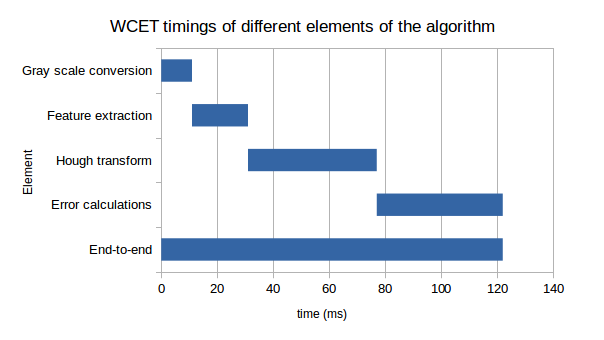
\includegraphics[width=1\linewidth]{./img/WCET_timings.png}
    \caption{\label{fig:WCET timings}WCET timings}
  \end{subfigure}
  \caption{\label{fig:Average and WCET timings of the different elements in the algorithm}Average and WCET timings of the different elements in the algorithm}
\end{figure}

Figure \ref{fig:Average and WCET timings of the different elements in the algorithm} shows how long time the different elements of the lane detection algorithm takes. In the test the smaller resolution of 384x288 was used. In \ref{fig:Average timings} it is clear that it is the image processing parts that consume the largest amount of time. Figure \ref{fig:WCET timings} shows the worst-case execution time for the same elements.\\




\begin{figure}[H]
  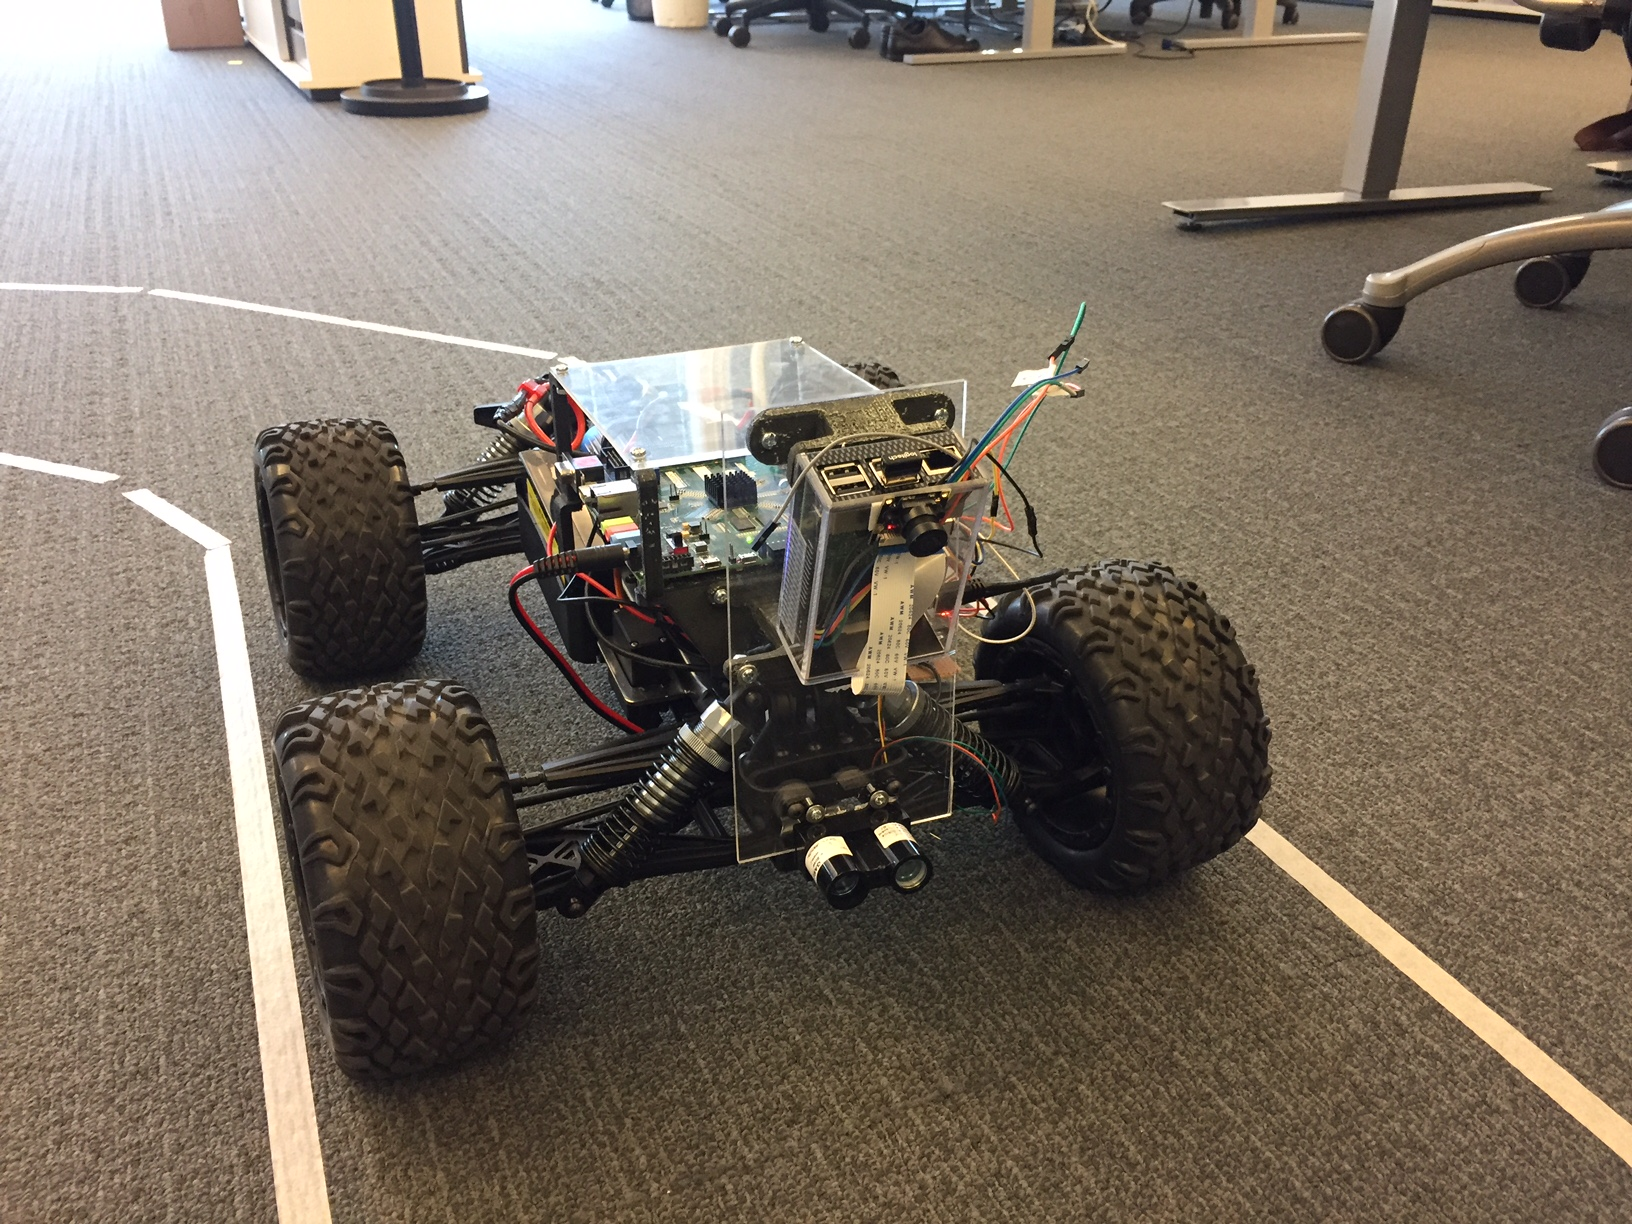
\includegraphics[width=\textwidth]{./img/utor.JPG}
  \centering
  \caption{The modified RC-car}
  \label{fig:The modified RC-car used for demonstrator}
\end{figure}

The figure \ref{fig:The modified RC-car used for demonstrator} above shows the demonstator vehicle with the mounted LIDAR and Raspberry Pi with camera. The main board behind the Raspberry is a Zedboard with the Xilinx Zynq-7000 chip.\\

